\documentclass[border=2pt]{standalone}
\usepackage{tikz}
\usetikzlibrary{angles,quotes}
\begin{document}
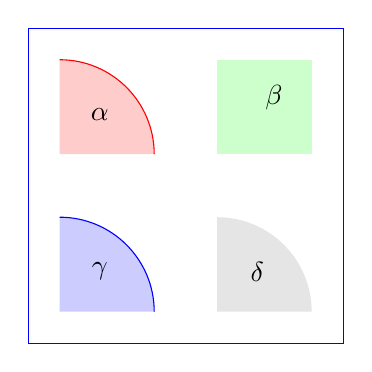
\begin{tikzpicture}[angle radius=1.2cm]
  \draw[blue] (-.4,-2.4) rectangle (3.6,1.6);
  \coordinate (O) at (0,0);
  \coordinate (A) at (1,0);
  \coordinate (B) at (0,1);
  \coordinate (P) at (2,0);
  \coordinate (C) at (3,0);
  \coordinate (D) at (2,1);
  \coordinate (Q) at (0,-2);
  \coordinate (E) at (1,-2);
  \coordinate (F) at (0,-1);
  \coordinate (R) at (2,-2);
  \coordinate (G) at (3,-2);
  \coordinate (H) at (2,-1);
  \pic[draw=red,fill=red!20,"$\alpha$"] {angle=A--O--B};
  \path pic[fill=green!20,"$\beta$"] {right angle=C--P--D};
  \path pic[draw=blue,fill=blue!20,"$\gamma$"] {angle=E--Q--F};
  \path pic[draw=none,fill=gray!20,"$\delta$"] {angle=G--R--H};
\end{tikzpicture}
\end{document}
